\documentclass{article}

\usepackage{tikz}
\usetikzlibrary{patterns}

\definecolor{pantoneblack7}{RGB}{62,62,59}
\definecolor{pantone144}{cmyk}{0,0.5,1,0}
\definecolor{pantone289}{cmyk}{1,0.6,0,0.56}

\tikzset{candidate/.style={draw, align=center, rounded corners=0.1cm, fill=white}}
\tikzset{balanced/.append style={draw=pantone144, thick, fill=pantone144!40}}
\tikzset{todo/.append style={draw=pantone144, thick, pattern=north west lines, pattern color=pantone144!40}}
\tikzset{target/.style={align=center, draw, thick, fill=white}}

\usepackage{pgfplots}

% Code from Christian Feuersänger
% http://tex.stackexchange.com/questions/54794/using-a-pgfplots-style-legend-in-a-plain-old-tikzpicture#54834

% argument #1: any options
\newenvironment{customlegend}[1][]{%
    \begingroup
    % inits/clears the lists (which might be populated from previous
    % axes):
    \csname pgfplots@init@cleared@structures\endcsname
    \pgfplotsset{#1}%
}{%
    % draws the legend:
    \csname pgfplots@createlegend\endcsname
    \endgroup
}%

% makes \addlegendimage available (typically only available within an
% axis environment):
\def\addlegendimage{\csname pgfplots@addlegendimage\endcsname}

\usepackage[scaled]{berasans}
\renewcommand*\familydefault{\sfdefault}  %% Only if the base font of the document is to be sans serif
\usepackage[T1]{fontenc}

\usepackage{cleveref}

\begin{document}
\begin{figure}[h]
  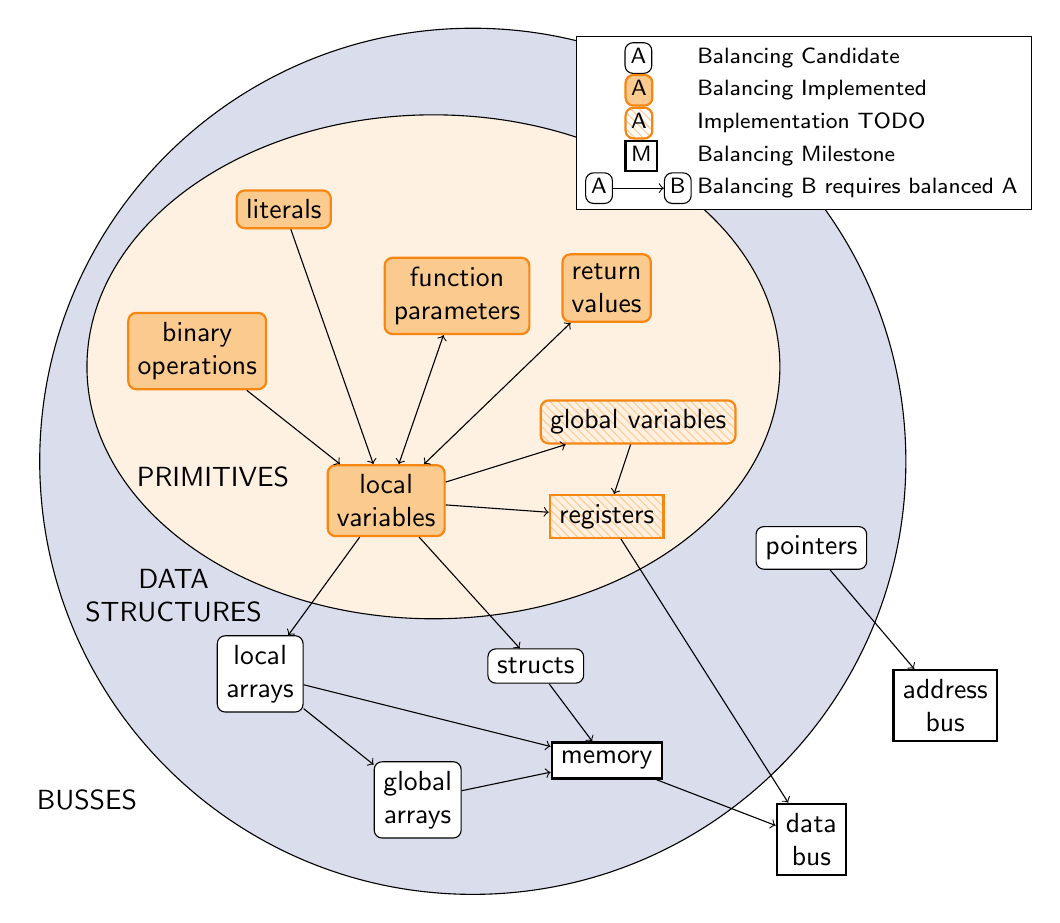
\begin{tikzpicture}
    \draw[fill=pantone289!10] (0.9, 0.1) ellipse (5.5cm and 5.5cm);
    \node[align=center] at (-2.9, -1.6) {DATA \\ STRUCTURES};

    \draw[fill=pantone144!10] (0.4,1.3) ellipse (4.4cm and 3.2cm);
    \node at (-2.4, -0.1) {PRIMITIVES};

    \node at (-4.0, -4.2) {BUSSES};

    \node (literals) [candidate, balanced] at (-1.5,3.3) {literals};
    \node (ops) [candidate, balanced] at (-2.6,1.5) {binary \\ operations};
    \node (lvars) [candidate, balanced] at (-0.2,-0.4) {local \\ variables};
    \node (gvars) [candidate, todo] at (3.0,0.6) {global variables};
    \node (params) [candidate, balanced] at (0.7, 2.2) {function \\ parameters};
    \node (returns) [candidate, balanced] at (2.6, 2.3) {return \\ values};
    \node (registers) [target, todo] at (2.6, -0.6) {registers};

    \draw[->] (literals) -> (lvars);
    \draw[->] (ops) -> (lvars);
    \draw[<->] (lvars) -> (params);
    \draw[<->] (lvars) -> (returns);
    \draw[->] (lvars) -> (gvars);
    \draw[->] (gvars) -> (registers);

    \draw[->] (lvars) -> (registers);

    \node (larrs) [candidate] at (-1.8, -2.6) {local \\ arrays};
    \node (garrs) [candidate] at (0.2, -4.2) {global \\ arrays};
    \node (structs) [candidate] at (1.7, -2.5) {structs};
    \node (memory) [target] at (2.6, -3.7) {memory};
    \node (pointers) [candidate] at (5.2, -1.0) {pointers};

    \draw [->] (lvars) -> (larrs);
    \draw [->] (larrs) -> (garrs);
    \draw [->] (lvars) -> (structs);
    \draw [->] (larrs) -> (memory);
    \draw [->] (garrs) -> (memory);
    \draw [->] (structs) -> (memory);

    %\draw [->, red, dashed] (memory) -> (registers);

    \node (databus) [target] at (5.2, -4.7) {data \\ bus};
    \node (addressbus) [target] at (6.9, -3.0) {address \\ bus};

    \draw[->] (registers) -> (databus);
    \draw[->] (memory) -> (databus);
    \draw[->] (pointers) -> (addressbus);

    \begin{customlegend}[legend cell align=left, legend entries={Balancing Candidate,Balancing Implemented,Implementation TODO,Balancing Milestone, Balancing B requires balanced A},
      %legend image post style={scale=2.3},
      legend style={at={(8,5.5)},font=\footnotesize}]
      \addlegendimage{legend image code/.code={\node[candidate] {A};}}
      \addlegendimage{legend image code/.code={\node[candidate, balanced] {A};}}
      \addlegendimage{legend image code/.code={\node[candidate, todo] {A};}}
      \addlegendimage{legend image code/.code={\node[target] {M};}}
      \addlegendimage{legend image code/.code={\node[candidate] (A) at (-0.5, 0) {A};\node[candidate] (B) at (0.5,0){B}; \draw[->] (A) -> (B);}}
    \end{customlegend}
  \end{tikzpicture}
  \caption{Balancing dependencies in LLVM}
  \label{fig:balancing}
\end{figure}
\end{document}
